<<echo=FALSE, cache=FALSE>>=
set_parent('./project.Rnw')
@
\section{Boosting}
\label{sec:Boosting}
%%fakesubsection Boosting
In this part boosting will be discussed, first in general terms with \textit{Adaboost} as an introductory example. The main focus will be on boosting trees and their performance, hereunder mainly \textit{Gradient boosting}.

The idea behind boosting is to combine many ''weak'' classifiers to create one ''strong''. This is usually referred to as a committee-based classifier, and bears some resemblance to other committee-based approaches such as \textit{bagging} as will be discussed in Section~\ref{sec:Bagging}.  Roughly said, the algorithms trains weak classifiers sequentially, and for each new classifier the data points are weighted by how hard they were for previous classifiers to classify correctly. At the end all the classifiers are combined and weighted based on how well they preform. The idea is better illustrated in Freund and Schapire's (1997) algorithm \textit{AdaBoost.M1} \cite{adaboostM1}.
\subsection{Adaboost}
\label{sub:Adaboost}
\todo{Adaboost or AdaBoost}
Adaboost.M1 \url{http://cseweb.ucsd.edu/~yfreund/papers/IntroToBoosting.pdf} This is mentioned in the start of boosting \cite{modstat} \\
\colorbox{yellow}{Some say it is sensitive to noisy data and outliers}\\
\colorbox{yellow}{Something about how boosting decrease bias. By tuning tree size, you can control the bias variance tradeoff.}\\
\\
Adaboost.M1 was created in (1997) and \colorbox{yellow}{some history}. Hastie et al. (2006) \cite{modstat} described it as the ''the most popular boosting algorithm'', and Breiman (1996) \cite{Breiman1996} as ''the best of-the-shelf classifier in the world'' . Only the two class case will be discussed here, but it generalizes easily. The method requires, both for two class and multi class, that the weak classifiers has prediction error less than $1/2$.

Consider output variable coded as $Y \in \{-1, 1\}$. A weak classifier $C(X)$ is chosen to do the ground work. This can for instance be a shallow tree, or some other algorithm that does not perform much better than random guessing. All the data points $\mathbf{x}_i$, $i = 1, 2, \ldots, N$, are initialized with weights $w_i = 1/N$. Then, for $m = 1$, $C_m(\mathbf{x}_i)$ is trained using the weights. $err_m$ is used as a performance measure for $C_m(\mathbf{x}_i)$.
\begin{align}
  err_m =  \frac{\sum^{N}_{i=1} w_i I\{y_i \neq C_m(\mathbf{x}_i)\}}{\sum^{N}_{i=1} w_i}.
\end{align}
Then the weights are updated using 
\begin{align}
  w_i &\leftarrow w_i \exp\left( \alpha_m I\{y_i \neq C_m(\mathbf{x}_i)\} \right), \\
  &\text{where} \quad \alpha_m = \log\left(  \frac{1-err_m}{err_m} \right).
\end{align}
This is repeated for $m = 1, \ldots, M$. Finally the classifier is created
\begin{align}
  C( \mathbf{x}) = \text{sign}\left( \sum^{M}_{m=1} \alpha_m C_m(\mathbf{x}) \right).
\end{align}
There are many choices of weak classifiers, but one of the more common is to use classification trees. It is then important to not grow an optimal tree as with CART, but instead grow a shallow tree or just stumps (one split). The size of the individual trees will be discussed in Section~\ref{sub:Tree size}. For computational purposes,the trees are only grown and not pruned back.
An example of this implementation can be found in the r package \verb+adabag+ \cite{adabag}. 

\subsection{Forward stagewise Additive Modeling}
\label{sub:Forward stagewise additive modeling}
A common way to view the goal of classification problems is through the expected prediction error (Appendix~\ref{sub:EPE}). The goal is to find
\begin{align}
  \label{eq:fargmin} 
  f^* = \argmin_f \E_{Y, X}[L(Y,F(X))] = \argmin_f \E_Y [L(Y,f(X))|X] ,
\end{align}
where $L(Y, f(X))$ is some loss function. Note that $L$ does not necessarily need to be the misclassification rate, but can be a continuous loss like squared-error loss, $(Y - f(X))^2$. As $f^*$ is usually hard to obtain, a common procedure is restrict $f$ to be a member of a parameterized class of function. In this section $f$ will be an additive expansion in a set of elementary basis functions 
\begin{align}
  \label{eq:additive} 
  f(\mathbf{x}) =  \sum^{M}_{m=1} \beta_m h(\mathbf{x}; \bm{\gamma}_m).
\end{align}
Here $h$ is usually a simple function of $\mathbf{x}$ an parameters $\bm{\gamma}$. These expansions are used in many different learning techniques like neural networks, wavelets, MARS and support vector machines.

Under \eqref{eq:additive}, the solution of \eqref{eq:fargmin} is usually still hard to obtain. Therefor \textit{forward stagewise additive modelling} approximates the solution by sequentially adding new basis functions without changing parameters of basis functions already fitted. The algorithm works the following way:\\
\\
$f_0$ is initialized to 0. For $m = 1, \ldots, M$, $\beta_m$ and $\bm \gamma_m$ is found by
\begin{align}
  \label{eq:forStageWise} 
  (\beta_m, \bm \gamma_m) = \argmin_{\beta, \bm \gamma} \sum^{N}_{i=1} L(y_i, f_{m-1}(\mathbf{x}_i) + \beta h(\mathbf{x}_i; \bm \gamma)).
\end{align}
Then $f_m(\mathbf{x})$ is updated to $f_m(\mathbf{x}) = f_{m-1}(\mathbf{x}) + \beta_m h(\mathbf{x}; \bm \gamma_m)$.\\
\\
If the basis functions are set to be a classifier $h(\mathbf{x}; \bm \gamma) \in \{-1, 1\}$, and the loss is exponential
\begin{align}
  \label{eq:expLoss} 
  L(y, f(\mathbf{x})) = \exp (-y f(\mathbf{x})),
\end{align}
it is pretty straight forward to show \cite{modstat} that forward stagewise modeling is equivalent to the Adaboost.M1 classifier in the previous section. This was not the original motivation for Adaboost.M1. The way Adaboost.M1 fits in the forward stagewise framework, was only discovered years later. However, the forward stargewise framework give the opportunity to compare the Adaboost.M1 to different loss functions. Under the exponential loss in \eqref{eq:expLoss}, the solution of \eqref{eq:fargmin} is 
\begin{align}
  f^*( \mathbf{x}) = \frac{1}{2} \log \frac{P(Y=1 |X=x)}{P(Y=-1 | X = x)} .
\end{align}
So the classification rule in Adabost.M1 approximates one half of the log-odds. That justifies using its sign as a classification rule.
%
\subsubsection{Loss functions}
\label{sub:Loss functions}
<<lossFunctions, echo=FALSE>>=
# Plot of different loss functions
source("../code/lossFunctions.R")
@
The choice of loss function is important in terms of both accuracy and computations. While the use of $0/1$ loss might be intuitive, a differentiable loss function might have a computational advantage. By using squared-error loss, $L = (Y - f(X))^2$, \eqref{eq:forStageWise} fit a basis function to the residual of the previous function. There exist fast algorithms for solving these type of problems, but squared-error loss is still not considered a good choice for classification. That can be explained by Figure~\ref{fig:lossFunctions}. The figure shows the loss $L(y, f(\mathbf{x}))$ for different loss functions, where $y \in \left\{ -1, 1 \right\}$. If the classification rule is $C(\mathbf{x}) = \mathrm{sign}(f(\mathbf{x}))$, then a positive margin $y f(\mathbf{x}) > 0$ implies a correct classification, while a negative margin implies a wrong. It is clear from the figure that squared-error loss start increasing when the margin is higher than $1$. As any loss function should penalize a negative margin more than a positive one, this makes squared-error loss not very well suited for classification.

From the figure it is clear that exponential and misclassification loss decrease with the margin and are therefore better choices than square-error loss. But as mentioned earlier, and will become more clear in Section~\ref{sub:Gradient boosting}, a differentiable loss gives some computational advantages. The last loss function in Figure~\ref{fig:lossFunctions} is the \textit{negative binomial log-likelihood}, or \textit{binomial deviance},
\begin{align}
  L(y, f(\mathbf{x})) = \log \left( 1 + \exp (-2 y f(\mathbf{x})) \right).
\end{align}
This locks very similar to the exponential loss, but might be the preferred choice. The main difference is that for increasingly negative margins the exponential loss penalize exponentially, while the binomial deviance penalize linearly. Therefore the binomial deviance is not as vulnerable in noisy settings. The binomial deviance is a very common choice and will be the main focus for the rest of Section~\ref{sec:Boosting}. 

For multi class cases, the binomial deviance generalizes to the \textit{multinomial deviance}
\begin{align}
  \label{eq:multinomialDeviance} 
  &L(y, \mathbf{f}( \mathbf{x })) = - \sum^{K}_{k=1} I\{y = k\} \log p_k(\mathbf{x}), \\
  \label{eq:multinomialDevianceProb} 
  &\text{where} \quad p_k(\mathbf{x}) = \frac{\exp (f_k(\mathbf{x}))}{\sum^{K}_{k=1} \exp (f_l(\mathbf{x}))}\\
  &\text{and} \quad \mathbf{f} = (f_1, \ldots, f_K)^T.
\end{align}
As with logistic regression, this is a probabilistic classifier, ie. it returns class probabilities. That is very useful in fields like data mining, but can also be useful in pure classification when combining into ensembles. \colorbox{yellow}{Need to mention ensemble learning somewhere.}

Zhu et al. (2009) \cite{zhu2009} generalize the exponential loss for multiple classes.
%
\begin{figure}[h!]
\begin{center}
    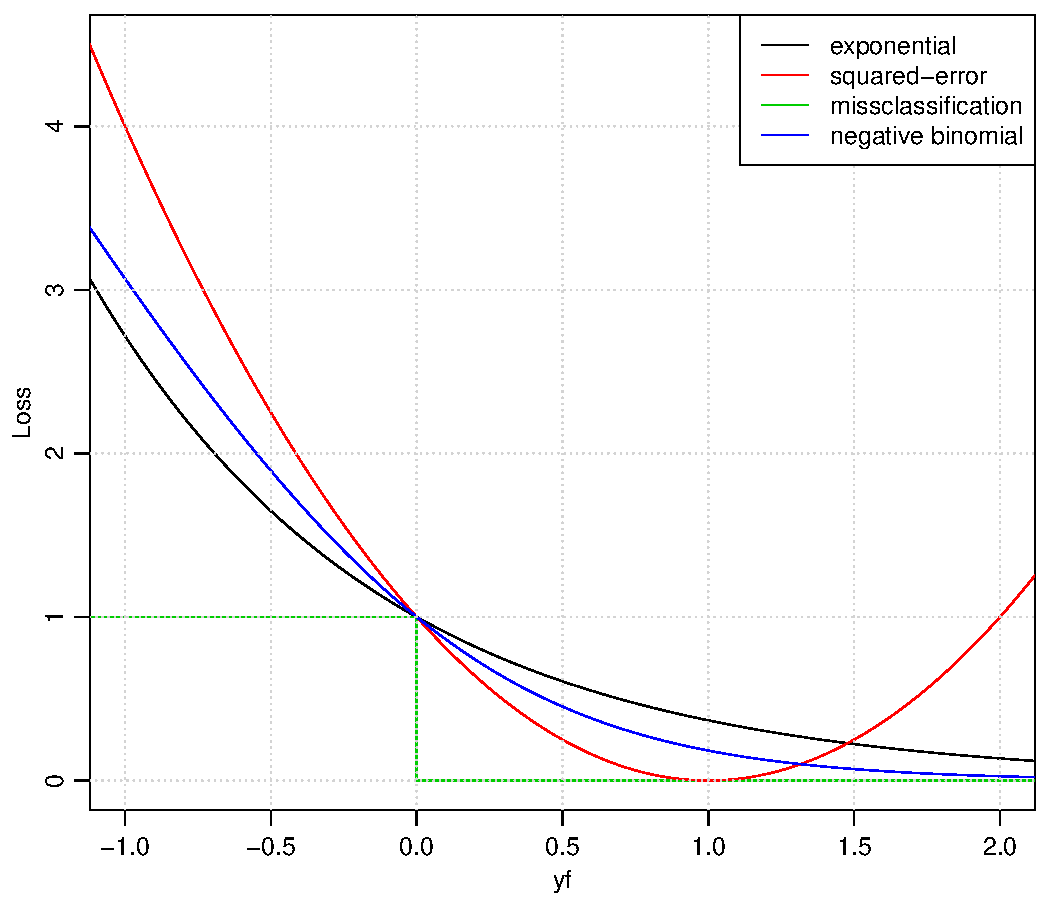
\includegraphics[scale=0.5]{./figures/lossFunctions.pdf}
\end{center}
\caption{Different loss functions $L(y, f)$ as function of the margin $yf$, scaled so all goes through point $(0, 1)$. $y \in \{-1, 1\}$.}
\label{fig:lossFunctions}
\end{figure}
%
\subsection{Gradient boosting}
\label{sub:Gradient boosting}
%%fakesubsubsection Gradient boosting
Gradient boosting paper \cite{friedman}. \colorbox{yellow}{Algo 6 is equal to algo 5  for K = 2}\\
Zhu et al. (2005) generalize exponential loss for K-class problems \cite[p.~349]{modstat}.

\colorbox{yellow}{Look at influence trimmin \cite{friedman}}.
\\
\\Gradient boosting is a smart method developed by Jerome H. Friedman (1999) \cite{friedman}. It is built on the stagewise fashion for arbitrary differentiable loss functions. The idea behind the method is to solve for $f^*$ \eqref{eq:fargmin} numerically, using steepest decent in function space.

Let $g_m$ denote the gradient at step $m$
\begin{align}
  g_{m}(\mathbf{x}) = \left[ \frac{\partial \E_{Y} \left[ L(Y, f(\mathbf{x})) \right | \mathbf{x}]}{\partial f(\mathbf{x})}  \right]_{f(\mathbf{x}) = f_{m-1}(\mathbf{x})},
\end{align}
or assuming sufficient regularity that integration and differentiation can be interchanged, 
\begin{align}
  g_{m}(\mathbf{x}) = \E_{Y} \left[ \frac{\partial L(Y, f(\mathbf{x})) }{\partial f(\mathbf{x})}  | \mathbf{x}\right]_{f(\mathbf{x}) = f_{m-1}(\mathbf{x})}.
\end{align}
$f_m$ is then updated to
\begin{align}
  f_m(\mathbf{x}) = f_{m-1}(\mathbf{x}) - \rho_m  g_m(\mathbf{x}),
\end{align}
where $\rho_m$ is the step length found by
\begin{align}
  \rho_m = \argmin_{\rho}  \E_{Y} \left[ L(Y, f_{m-1}(\mathbf{x}) - \rho g_m(\mathbf{x})) \right | \mathbf{x}].
\end{align}
By repeating these steps, the function is moving towards a minimum of $L$ (in the steepest decent direction $-g_m$), though in a very greedy matter. \\
\\
In the steepest decent algorithm above above $\mathbf{x}$ is considered a stochastic variable, but that is not really the case. For finite data $(\mathbf{x}_i, y_i)$ for $i = 1, \ldots, N$, $E_Y \left[\: \cdot \:| \mathbf{x} \right]$ can not be accurately estimated by the data values, and is only defined at the training points. As the goal is to find a good approximation for $f^*(\mathbf{x})$ for all $\mathbf{x}$, a different approach is needed. Friedman's approach to tackle this was to impose an additive parameterized form of $f$ as in \eqref{eq:additive}, and do parameter optimization over those constraints. By doing the fitting in a stagewise matter, the optimization problem was reduced to the forward stagewise additive modeling problem \eqref{eq:forStageWise}. As this is often difficult to solve, he approximated a solution based on the steepest decent algorithm.

For a given $f_{m-1}(\mathbf{x})$, the function $\beta_m h(\mathbf{x}; \bm{\gamma}_m)$ can be viewed as the best step toward the databased $f^*$, under the given constraint \eqref{eq:additive}, and is can therefore be considered a steepest decent step. It is often hard to find the solution to \eqref{eq:forStageWise}, but as $\beta_m h(\mathbf{x}; \bm{\gamma}_m)$ is comparable to the unconstrained negative gradient $g_m$, it can be fitted to $-g_m$ instead. This is done by finding the $\beta_m h(\mathbf{x}; \bm{\gamma}_m)$ highest correlated to $-g_m(\mathbf{x})$,
\begin{align}
  \label{eq:gradBoostFit} 
  \bm \gamma_m = \argmin_{\beta, \bm \gamma} \sum^{N}_{i=1} \left( -g_m(\mathbf{x}_i) - \beta h(\mathbf{x}_i; \bm \gamma) \right)^2.
\end{align}
Then $f_m$ is updated using
\begin{align}
  &f_m(\mathbf{x}) = f_{m-1}(\mathbf{x}) + \rho_m h(\mathbf{x}; \bm{\gamma}_{m}),\\
  \label{eq:lineSearch} 
  &\text{where} \quad \rho_m = \argmin_\rho \sum^{N}_{i=1} L(y_i, f_{m-1}(\mathbf{x}) + \rho h(\mathbf{x}; \bm{\gamma}_m)).
\end{align}
These last three equations are know as the \textit{gradient boosting algorithm}.
As \eqref{eq:forStageWise} is replaced by \eqref{eq:gradBoostFit}, $\tilde{y}_i = -g_m(\mathbf{x}_i)$ is often referred to as the ''pseudo-responce''. 
Note here that $h$ and $f$ are continuous functions and not classifiers. The classification is done after all the $M$ iterations, usually trough some relationship between $f_M$ and class probabilities. For the binomial deviance loss this relationships are the log-odds,
\begin{align}
  \label{eq:boostLogOdds1} 
  &\hat P(Y = 1 |  \mathbf{x}) = \left( 1+ \exp\left( -2 f_M (\mathbf{x}) \right) \right)^{-1},\\
  \label{eq:boostLogOdds2} 
  &\hat P(Y = -1 |  \mathbf{x}) = \left( 1+ \exp\left( 2 f_M (\mathbf{x}) \right) \right)^{-1}.
\end{align}
Later it will be show how powerful this simple algorithm is, but first trees will be used as the basis functions $\beta_m h(\mathbf{x}; \bm{\gamma}_m)$.

\subsubsection{Regression Trees}
\label{sub:Regression Trees}
It was earlier mentioned that the basis functions $h(\mathbf{x}; \bm{\gamma}_m)$ in gradient boosting are continuous functions. Therefore, classification trees can not be used and the regression framework needs to be explored.
In section \ref{sub:Classification trees} it was show how classification trees can be fitted using the CART method. CART stands for \textit{Classification And Regression Trees} and can obviously also be used for regression. The ides behind fitting regression trees are almost identical to classification, but the functions used during growing, estimating and pruning are different. However, this will not be investigated deeply, only what is needed in the boosting framework.\\
\\
A regression tree $T$ can be represented in the following form 
\begin{align}
  T(\mathbf{x}; \left\{ c_j, R_j \right\}_{j = 1}^J)  = \sum^{J}_{j=1} c_j I\left\{ \mathbf{x} \in R_j \right\}.
\end{align}
As with classification all the regions $R_j$ are disjunct and collectively cover all possible values of $\mathbf{x}$. If fitting a tree to the response $\tilde y$ under squared error loss, it is straight forward to see that the solution in each region $R_j$ is just the region average
\begin{align}
  \hat{c}_j = \mathrm{ave}(\tilde y_i | \mathbf{x}_i \in R_j).
\end{align}
The tree is grown sequentially, similarly as with classification, by finding the split that minimize the total squared error loss. When a larger tree is grown, it can then be pruned back using \textit{const-complexity pruning} based on the squared error and penalized by the number of terminal nodes. In the boosting context however, pruning is not really an alternative. Usually $J \leq 10$ end-nodes will be sufficient \cite[p.~363]{modstat}, and thus growing a larger tree and pruning it back will only be very computationally expensive without much effect on the end results. The tree size will be further discussed in Section~\ref{sub:Tree size}.\\
\\
In gradient boosting trees are fitted in \eqref{eq:gradBoostFit}, in place of $\beta h(\mathbf{x}_i; \bm{\gamma})$ and $f_m$ can be created by
\begin{align}
  f_m(\mathbf{x}) = f_{m-1}(\mathbf{x}) + \rho_m T(\mathbf{x}; \left\{ c_{m j}, R_{m j} \right\}_{j=1}^{J}),
\end{align}
where $\rho_m$ is the solution of the line search in \eqref{eq:lineSearch}.  However, what is more common is to use one variable $\eta_{m j}$ instead of $\rho_m c_{m j}$. Thus $J$ separate basis functions are fitted instead of one single additive. This gives the opportunity to better tune the coefficients and improving the fit. So $f_m$ is set to 
\begin{align}
  \label{eq:etaLineSearch} 
  f_m(\mathbf{x}) = f_{m-1}(\mathbf{x}) +  \sum^{J}_{j=0} \eta_{m j} I\left\{ \mathbf{x} \in R_{m j} \right\}.
\end{align}
As the trees are disjunct, each $\eta_{m j}$ can be found independently.
\begin{align}
  \eta_{m j} = \argmin_\eta  \sum_{\mathbf{x}_i \in R_{m j}} L(y_i, f_{m-1}(\mathbf{x}) + \eta).
\end{align}

\subsubsection{The two-class logistic regression classifier}
\label{sub:The two-class logistic regression classifier}
The framework for gradient boosting is now reviewed, and the final step is to summarize the algorithm under binomial deviance loss. As before $y \in \left\{ -1, 1 \right\}$ and the loss is 
\begin{align}
  &L(Y, f(\mathbf{x})) = \log (1 + \exp (-2 Y f(\mathbf{x}))),\\
  &\text{where} \quad f(\mathbf{x}) = \frac{1}{2} \log \frac{ P(Y = 1 | \mathbf{x})}{ P(Y = -1 | \mathbf{x})}  .
\end{align}
$f_0(\mathbf{x})$ is initialized to $\frac{1}{2} \log \frac{1+\bar{y}}{1-\bar{y}}$.  The ''pseudo-responce'' is
\begin{align}
  \label{eq:ytildeGradboost} 
  &\tilde{y}_i = 
  -\left[ \frac{\partial L(y_i, f(\mathbf{x}_i)) }{\partial f(\mathbf{x}_i)}  \right]_{f(\mathbf{x}) = f_{m-1}(\mathbf{x})}
  = 2 y_i / (1 + \exp \left( 2 y_i f_{m-1}(\mathbf{x}_i) \right), \quad i = 1, \ldots, N.
\end{align}
A regression tree $T$ is fitted to $\tilde y_i$,
\begin{align}
  \left\{ R_{m j} \right\}_{j = 1}^J  = 
  \argmin_{\left\{ c_j, R_{j} \right\}_{j = 1}^J} \sum^{N}_{i=1} \left( \tilde y_i - T(\mathbf{x}_i; \left\{ c_j, R_j \right\}_{j = 1}^J) \right)^2.
\end{align}
The line searches in \eqref{eq:etaLineSearch} becomes
\begin{align}
  \eta_{m j} = \argmin_\eta  \sum_{\mathbf{x}_i \in R_{m j}} \log (1 + \exp [-2 y_i (f_{m-1}(\mathbf{x}_i) + \eta) ]), \quad j = 1, \ldots, J,
\end{align}
but this expression has no closed form solution. A common way to approximate the solution is by doing a Newton-Raphson step instead \cite{friedman}.
\begin{align}
  \eta_{m j} =  \frac{\sum_{\mathbf{x}_i \in R_{m j}} \tilde y_i}{\sum_{\mathbf{x}_i \in R_{m j}} |\tilde y_i|(2-|\tilde y_i|)}.
\end{align}
Here  $\tilde y_i$ is found in \eqref{eq:ytildeGradboost}. $f$ can now be updated by
\begin{align}
  \label{eq:gradBoostUpdateF} 
  f_m(\mathbf{x}) = f_{m-1}(\mathbf{x}) +  \sum^{J}_{j=0} \eta_{m j} I\left\{ \mathbf{x} \in R_{m j} \right\}.
\end{align}
All this is repeated $M$ times, and classification can be done based on the log-odds, as mentioned in \eqref{eq:boostLogOdds1} and \eqref{eq:boostLogOdds2}. \\
\\
It is pretty straight forward to expand the algorithm to multi-class classification. As mentioned earlier, the binomial deviance generalizes to the multinomial deviance in \eqref{eq:multinomialDeviance}. As there are now $K$ functions $f_k$, $K$ different trees has to be fitted at each iteration, on for each pair $(\tilde y_{k i}, f_k)$.Correspondingly, $J$ coefficients $\eta_{m k j}$ has to be fit for each tree, using the Newton-Raphson step. At he end the classifier is created based on the estimated class probabilities in \eqref{eq:multinomialDevianceProb}. For more details see for example \cite{friedman}.

\subsection{Tuning boosting algorithms}
\label{sub:Tuning boosting algorithms}
As mentioned earlier, the boosting algorithms have parameters that need to be set by the user. The choice of these parameters can have a great impact on both performance and time, and they often depend on each other. The first parameter that might come to mind is the number of boosting iterations $M$. It controls the balance between underfitting and overfitting. The choice for $M$ is usually made through either a test set, if there is a large amount of data, or through cross-validation. It is also possible to use the \textit{Out-of-bag} estimates for  \textit{Stochastic gradient boosting} (see Section~\ref{sub:Stochastic gradient boosting}, and \todo{ref to OOB}), which will be discussed later. 

\subsubsection{Tree size}
\label{sub:Tree size}
\colorbox{yellow}{Write somewhere how I use the term ''bias-variance tradeoff'', even though it does not apply to classification. }\\
\colorbox{yellow}{This is because it as similar properties, although not as easy to show.}\\
\colorbox{yellow}{Find some references of people that have tried (phd thesis), or here}\\
\url{http://homes.cs.washington.edu/~pedrod/papers/kdd97.pdf}\\ 
\colorbox{yellow}{This url is good, even though it was written for bagging.}\\
The number of terminal nodes $J$ in the trees controls the classification equivalence of a ''bias-variance tradeoff'' discussed in \colorbox{yellow}{section}. Large trees has high variance and low bias, while small trees have the opposite.   Following the reasoning in \cite{modstat} and \cite{friedman}, the goal is to find $f^*$ solving \eqref{eq:fargmin}. Consider an ANOVA expansion of the solution,
\begin{align}
  \label{eq:ANOVAexpansion} 
  f^*(\mathbf{x}) = \sum_{i} f_i(x_i) + \sum_{ij} f_{ij}(x_i, x_j) + 
  \sum_{ijk} f_{ijk}(x_i, x_j, x_k) + \cdots,
\end{align}
where $\mathbf{x} = (x_1, x_2, \ldots, x_p)^T$. $f_i$ is called the ''main-effect'', $f_{ij}$ the ''second order interaction'', $f_{ijk}$ the ''third order interaction'', and so on. The expansion is such that the first sum is the best approximation to $f^*$ under the constraint of only ''main-effects''. The second sum gives the best approximation of $f^*$ under the constrain of only ''main-effects'' and ''second order interactions''. This way \eqref{eq:ANOVAexpansion} can be viewed as an additive model. 

When fitting an additive model of trees with only two terminal nodes (commonly called stumps), these will have the same structure as the ''main-effects''. To capture interactions of order up to $J$, a tree with $J+1$  terminal nodes is needed, in addition to $N>J$. However, by setting $J$ to large, unnecessary variance is introduced in the trees. Boosting methods works by lowering the bias through the forward stagewise process, so it might be advantageous to use high bias low variance trees, but ideally one would of course try to be close to the dominant interaction order of $f^*$.
Experience suggest that $4 \leq J \leq 8$ usually works well, and $J>10$ is rarely needed \cite{modstat}.  

\subsubsection{Shrinkage}
\label{sub:Shrinkage}
As discussed earlier, regularization is controlled by number of boosting iterations $M$. However, test has shown  \cite{copas1983} that \textit{shrinkage} might improve the results obtained by only restricting on $M$. For the gradient boosting algorithm it is straight forward to include this. 
The update of $f$ in \eqref{eq:gradBoostUpdateF} is just changed to
\begin{align}
  f_m(\mathbf{x}) = f_{m-1}(\mathbf{x}) +  \nu \sum^{J}_{j=0} \eta_{m j} I\left\{ \mathbf{x} \in R_{m j} \right\}, \quad 0 < \nu < 1,
\end{align}
or more generally in the forward stagewise framework,
\begin{align}
  f_m(\mathbf{x}) = f_{m-1}(\mathbf{x}) +  \nu \: \beta_m h(\mathbf{x}; \bm \gamma_m), \quad 0 < \nu < 1.
\end{align}
Here $\nu$ is often referred to as the ''learning rate'' or ''shrinkage parameter''. Empirically it has been found \cite{friedman} that smaller values of $\nu$ give better test error. However, it requires a correspondingly larger $M$. This can be expensive as computations scales with $M$. This $\nu$-$M$ tradeoff will be illustrated in simulations.


\subsubsection{Influence trimming}
\label{sub:Influence trimming}
\todo{influence trimming \cite{friedman}?}
For binomial loss, at the $m$'th iteration, the problem at hand is to minimize
\begin{align}
  \label{eq:influence} 
  \sum_{i = 1}^{N} \log \left( 1 + \exp[ -2 y_i f_{m-1}(\mathbf{x}_i)] \exp [-2 y_i \rho h(\mathbf{x}_i; \bm \gamma)] \right),
\end{align}
over $\rho$ and $\bm \gamma$.  For $y_i f_{m-1}(\mathbf{x}_i)$ large, the effect of of $\rho h(\mathbf{x}_i; \bm{\gamma})$ is very small, and the minimization of \eqref{eq:influence} is more or less independent of $\rho h(\mathbf{x}_i; \bm \gamma)$. This means that the data point $(\mathbf{x}_i, y_i)$ can be removed from the calculations, without any substantial effect on $\rho$ and $\bm \gamma$. Removing such points during training is called \textit{influence trimming}, and can speed up the calculations. Friedman therefore proposed 
\begin{align}
  w_i = \exp (- 2 y_i f_{m-1}(\mathbf{x}_i)), 
\end{align}
as an measure for influence. 

More generally, the influence can be measured, by the second derivative of the loss function
\begin{align}
  w_i = \left[ \frac{\partial^2 L(y_i, f(\mathbf{x}_i)) }{\partial f(\mathbf{x}_i)^2}  \right]_{f(\mathbf{x}) = f_{m-1}(\mathbf{x})}.
\end{align}
This is because the first derivatibe is close to zero optimal values for $\rho$ and $\bm \gamma$, so the second derivative gives a more stable measurment.  For the binomial loss, this becomes 
\begin{align}
  w_i = |\tilde y_i| \: (2 - |\tilde y_i|). 
\end{align}
\todo{Check that this is correct.}
\colorbox{yellow}{Check that $|\tilde{y}_i|\: (2 - |\tilde{y}_i|)$ is correct.}\\
\\
Using this method Friedman suggest \cite{friedman} that this chould have an considerable impact on cumputing time, while leaving the estimates relatively untouched. 




\subsection{Variable selection}
\label{sub:Variable selection}
\colorbox{yellow}{Should at least mention something about variable selection. See \cite[sec. 8.1]{friedman}?}

\subsection{Interpretation}
\label{sub:Interpretation}
\colorbox{yellow}{Section on interpretation? See \cite[10.3]{modstat} and \cite{friedman}.}

\subsection{Stochastic gradient boosting}
\label{sub:Stochastic gradient boosting}
ada: an R package for stochastic boosting \url{http://dept.stat.lsa.umich.edu/~gmichail/ada_final.pdf} \\
\\
In 1996, Breiman \cite{Breiman1996} introduced his \textit{bagging} procedure, as will be further explained in  \colorbox{yellow}{sectionref}. He showed that the performance of function estimation procedures could be improved by introducing randomness in the training data. Inspired by this, in addition to Freund and Schapire's randomization of Adaboost in 1996 \cite{freund1996} and Breiman's hybrid procedure of boosting and bagging in 1999 \cite{breiman1999}, Friedman developed in 1999 the \textit{stochastic gradient boosting} algorithm \cite{FriedmanStochBoost}.
This new method is only a slight modification of the gradient boosting algorithm, but has been shown capable of outperforming its gradient boosting, both in terms of accuracy and computational speed  \cite{FriedmanStochBoost}.

The idea is: draw a random subsample of the training data, without replacement, at each iteration. All the steps are exactly the same as in the gradient boosting algorithm, but they are performed on the subsample. \\
\\
The size of the subset, $N_{sub}$, introduce another tuning parameter. Smaller values of $N_{sub}$ introduce more randomness to the procedure, while reducing computing time by the fraction $N_{sub}/N$. However, as the data trained on at each iterations becomes smaller, the variance of the individual base learners will increase. The gain comes from reduction in the correlation between estimates at each iteration, as this tend to reduce the variance of the combined model \eqref{eq:additive}.

For $N_{sub} = 0.5$, the algorithm is approximately equivalent to drawing bootstrap samples. Therefore, typical values used for $N_{sub}$ is around $0.5$ \cite{modstat}, but can be made substantially lower for larger datasets.

